\documentclass{anstrans}
%%%%%%%%%%%%%%%%%%%%%%%%%%%%%%%%%%%
\title{Coupled Neutronics and Microstructure Calculations to Model Energy Deposition and Radiation Damage in TREAT Fuel}
\author{Pedram Ghassemi$^1$, Sebastian Schunert$^2$, Daniel Schwen$^3$, Benjamin Baker$^4$, Adam Zabriskie$^5$, Javier Ortensi$^4$, Mark DeHart$^4$, Richard Martineau$^6$}
\institute{$^1$Department of Nuclear Engineering, North Carolina State University\\
               $^2$Nuclear Methods Development Group, Idaho National Laboratory, Idaho Falls, ID\\
	      $^3$XXX, Idaho National Laboratory, Idaho Falls, ID\\	
               $^4$Reactor Physics and Design Group, Idaho National Laboratory, Idaho Falls, ID\\
               $^5$Oregon State\\
               $^6$Modeling \& Simulation, Idaho National Laboratory, Idaho Falls, ID\\}

\email{pghasse@ncsu.edu, sebastian.schunert@inl.gov}

%%%% packages and definitions (optional)
\usepackage{graphicx} % allows inclusion of graphics
\usepackage{booktabs} % nice rules (thick lines) for tables
\usepackage{microtype} % improves typography for PDF
\usepackage{algorithm}
\usepackage{algorithmic}
\usepackage{mathtools}
\usepackage{amsmath}

%  various packages that you may wish to activate for usage
\usepackage{graphicx}
\usepackage{tabls}
\usepackage{afterpage}
\usepackage{amsmath}
\usepackage{amsfonts}
\usepackage{amssymb}
\usepackage{amstext}
\usepackage{amsbsy}
\usepackage{epsfig}
%\usepackage{cites}
\usepackage{epsf}
\usepackage{float} %utiliser H pour forcer � mettre l'image o� on ve

\usepackage{array}
{\usepackage{color}}
\usepackage[section]{placeins} % force � mettre l'image o� on veut
\usepackage{lscape} %utilisation du mode paysage
\usepackage{xspace}

%\usepackage[pdftex,bookmarks=true]{hyperref}
\usepackage{url}
\usepackage{verbatim}
%\usepackage[all]{hypcap}

\usepackage[labelsep=quad]{caption} % needed by the breakalgo environment

\usepackage{ifthen}
%\usepackage{subfig}

\usepackage{algorithmic}
\usepackage{algorithm}
\usepackage{listings}
\usepackage[noprefix]{nomencl}  % for nomenclature
%\usepackage[intoc]{nomencl}  % for nomenclature

%\usepackage{notebook2e, latexsym}
%
% de dk:
%
%%\usepackage[dvips]{epsfig}
%%\usepackage[dvips]{graphicx}
%%\usepackage{comment}
%%\usepackage{floatfig}
%%\usepackage{lscape}
%%\usepackage{landscape}
%%\usepackage{graphics}
%%\usepackage{hhline}[]
%%\usepackage{latexsym}
%%\usepackage{tabularx}[]
%%\usepackage{layout}
%
% de btp:
%
%%\usepackage{fancyheadings}
%%\usepackage{minitoc}
\usepackage{rotating}
%% \usepackage{rotate}
\usepackage{subfigure}
%%\usepackage{mathaccent}
%%\usepackage{isolatin1}
%
%%\usepackage{xspace}
%%\usepackage{longtable}
%%\usepackage{caption2}
%%\usepackage{ifthen}
%
\usepackage{mathpazo}
\usepackage{hyperref}

%
%=================================================================================================
% new commands
% +++++++++++++++++++++++++++++++++++++++++++++++++++++++++++++++++++++++++++++++++++++++++++++++++
\newcommand{\nc}{\newcommand}
%
% Ways of grouping things
%
\newcommand{\bracket}[1]{\left[ #1 \right]}
\newcommand{\bracet}[1]{\left\{ #1 \right\}}
\newcommand{\fn}[1]{\left( #1 \right)}
\newcommand{\ave}[1]{\left\langle #1 \right\rangle}
%
% Derivative forms
%
\newcommand{\dx}[1]{\,d#1}
\newcommand{\dxdy}[2]{\frac{\partial #1}{\partial #2}}
\newcommand{\dxdt}[1]{\frac{\partial #1}{\partial t}}
\newcommand{\dxdz}[1]{\frac{\partial #1}{\partial z}}
\newcommand{\dfdt}[1]{\frac{\partial}{\partial t} \fn{#1}}
\newcommand{\dfdz}[1]{\frac{\partial}{\partial z} \fn{#1}}
\newcommand{\ddt}[1]{\frac{\partial}{\partial t} #1}
\newcommand{\ddz}[1]{\frac{\partial}{\partial z} #1}
\newcommand{\dd}[2]{\frac{\partial}{\partial #1} #2}
\newcommand{\ddx}[1]{\frac{\partial}{\partial x} #1}
\newcommand{\ddy}[1]{\frac{\partial}{\partial y} #1}
%
% Vector forms
%
%\renewcommand{\vec}[1]{\ensuremath{\stackrel{\rightarrow}{#1}}}
%\renewcommand{\div}{\ensuremath{\vec{\nabla} \cdot}}
%\newcommand{\grad}{\ensuremath{\vec{\nabla}}}

\renewcommand{\div}{\vec{\nabla}\! \cdot \!}
\newcommand{\grad}{\vec{\nabla}}
\newcommand{\oa}[1]{\fn{\frac{1}{3}\hat{\Omega}\!\cdot\!\overrightarrow{A_{#1}}}}

%
% Equation beginnings and endings
%
\newcommand{\bea}{\begin{eqnarray}}
\newcommand{\eea}{\end{eqnarray}}
\newcommand{\be}{\begin{equation}}
\newcommand{\ee}{\end{equation}}
\newcommand{\beas}{\begin{eqnarray*}}
\newcommand{\eeas}{\end{eqnarray*}}
\newcommand{\bdm}{\begin{displaymath}}
\newcommand{\edm}{\end{displaymath}}
%
% Equation punctuation
%
\newcommand{\pec}{\hspace{0.25in},}
\newcommand{\pep}{\hspace{0.25in}.}
\newcommand{\pev}{\hspace{0.25in}}
%
% Equation labels and references, figure references, table references
%
\newcommand{\LEQ}[1]{\label{eq:#1}}
\newcommand{\EQ}[1]{Eq.~(\ref{eq:#1})}
\newcommand{\EQS}[1]{Eqs.~(\ref{eq:#1})}
\newcommand{\REQ}[1]{\ref{eq:#1}}
\newcommand{\LFI}[1]{\label{fi:#1}}
\newcommand{\FI}[1]{Fig.~\ref{fi:#1}}
\newcommand{\RFI}[1]{\ref{fi:#1}}
\newcommand{\LTA}[1]{\label{ta:#1}}
\newcommand{\TA}[1]{Table~\ref{ta:#1}}
\newcommand{\RTA}[1]{\ref{ta:#1}}

%
% List beginnings and endings
%
\newcommand{\bl}{\bss\begin{itemize}}
\newcommand{\el}{\vspace{-.5\baselineskip}\end{itemize}\ess}
\newcommand{\benu}{\bss\begin{enumerate}}
\newcommand{\eenu}{\vspace{-.5\baselineskip}\end{enumerate}\ess}
%
% Figure and table beginnings and endings
%
\newcommand{\bfg}{\begin{figure}}
\newcommand{\efg}{\end{figure}}
\newcommand{\bt}{\begin{table}}
\newcommand{\et}{\end{table}}
%
% Tabular and center beginnings and endings
%
\newcommand{\bc}{\begin{center}}
\newcommand{\ec}{\end{center}}
\newcommand{\btb}{\begin{center}\begin{tabular}}
\newcommand{\etb}{\end{tabular}\end{center}}
%
% Single space command
%
%\newcommand{\bss}{\begin{singlespace}}
%\newcommand{\ess}{\end{singlespace}}
\newcommand{\bss}{\singlespacing}
\newcommand{\ess}{\doublespacing}
%
%---New environment "arbspace". (modeled after singlespace environment
%                                in Doublespace.sty)
%   The baselinestretch only takes effect at a size change, so do one.
%
\def\arbspace#1{\def\baselinestretch{#1}\@normalsize}
\def\endarbspace{}
\newcommand{\bas}{\begin{arbspace}}
\newcommand{\eas}{\end{arbspace}}
%
% An explanation for a function
%
\newcommand{\explain}[1]{\mbox{\hspace{2em} #1}}
%
% Quick commands for symbols
%
\newcommand{\half}{\frac{1}{2}}
\newcommand{\third}{\frac{1}{3}}
\newcommand{\twothird}{\frac{2}{3}}
\newcommand{\fourth}{\frac{1}{4}}
\newcommand{\mdot}{\dot{m}}
\newcommand{\ten}[1]{\times 10^{#1}\,}
\newcommand{\cL}{{\cal L}}
\newcommand{\cD}{{\cal D}}
\newcommand{\cF}{{\cal F}}
\newcommand{\cE}{{\cal E}}
\renewcommand{\Re}{\mbox{Re}}
\newcommand{\Ma}{\mbox{Ma}}
%
% Inclusion of Graphics Data
%
%\input{psfig}
%\psfiginit
%
% More Quick Commands
%
\newcommand{\bi}{\begin{itemize}}
\newcommand{\ei}{\end{itemize}}
\newcommand{\ben}{\begin{enumerate}}
\newcommand{\een}{\end{enumerate}}
\newcommand{\dxi}{\Delta x_i}
\newcommand{\dyj}{\Delta y_j}
\newcommand{\ts}[1]{\textstyle #1}


\newcommand{\bu}{\boldsymbol{u}}
\newcommand{\ber}{\boldsymbol{e}}
\newcommand{\br}{\boldsymbol{r}}
\newcommand{\bo}{\boldsymbol{\Omega}}

\newcommand{\bn}{\boldsymbol{\nabla}}

% DGFEM commands
\newcommand{\jmp}[1]{[\![#1]\!]}                     % jump
\newcommand{\mvl}[1]{\{\!\!\{#1\}\!\!\}}             % mean value
\newcommand{\jmpa}[1]{[\![\![#1]\!]\!]}              % jump


\newcommand{\boxedeqn}[1]{%
  \[\fbox{%
      \addtolength{\linewidth}{-2\fboxsep}%
      \addtolength{\linewidth}{-2\fboxrule}%
      \begin{minipage}{\linewidth}%
      \begin{equation}#1\end{equation}%
      \end{minipage}%
    }\]%
}
\newcommand{\mboxed}[1]{\boxed{\phantom{#1}}}
\newcommand{\ud}{\,\mathrm{d}}

% keff
\newcommand{\keff}{\ensuremath{k_{\textit{eff}}}\xspace}

% margin par
\newcommand{\mt}[1]{\marginpar{ {\footnotesize #1} }}

% shortcut for aposterio in italics
\newcommand{\apost}{\textit{a posteriori\xspace}}
\newcommand{\Apost}{\textit{A posteriori}\xspace}

% shortcut for multi-group
\newcommand{\mg}{multigroup\xspace}
\newcommand{\Mg}{Multigroup\xspace}
\newcommand{\ho}{higher-order\xspace}
\newcommand{\Ho}{Higher-order\xspace}
\newcommand{\HO}{Higher-Order\xspace}
\newcommand{\HObig}{HIGHER-ORDER\xspace}
\newcommand{\Mgbig}{MULTIGROUP\xspace}
\newcommand{\sn}{$S_N$\xspace}
\newcommand{\pn}{$P_N$\xspace}

% shortcut for Rattlesnake
\newcommand{\rattlesnake}{Rattlesnake}

% shortcut for domain notation
\newcommand{\D}{\mathcal{D}}
\newcommand{\Sp}{\mathcal{S}}

% shortcut for xuthus
\newcommand{\psc}[1]{{\sc {#1}}}
\newcommand{\xuthus}{\psc{xuthus}\xspace}

% vector shortcuts
\newcommand{\vo}{\vec{\Omega}}
\newcommand{\vr}{\vec{r}}
\newcommand{\vn}{\vec{n}}
\newcommand{\vnk}{\vec{\mathbf{n}}}

% extra space
\newcommand{\qq}{\quad\quad}

% sign function
\DeclareMathOperator{\sgn}{sgn}


\makeatletter
\newcommand{\rmnum}[1]{\romannumeral #1}
\newcommand{\Rmnum}[1]{\expandafter\@slowromancap\romannumeral #1@}
\makeatother

\newcommand{\ensuretext}[1]{\ensuremath{\text{#1}}}
\newcommand{\Rmnumb}[1]{\ensuretext{\Rmnum{#1}}}

% common reference commands
\newcommand{\eqt}[1]{Eq.~(\ref{#1})}                     % equation
\newcommand{\fig}[1]{Fig.~\ref{#1}}                      % figure
\newcommand{\tbl}[1]{Table~\ref{#1}}                     % table
\newcommand{\app}[1]{Appendix~\ref{#1}}                  % appendix


% for mathematica notebook
\newcommand{\IndentingNewLine}{ \\ }


\newcommand{\rhs}{right-hand-side\xspace}
\newcommand{\clearemptydoublepage}{\newpage{\pagestyle{empty}\cleardoublepage}}

\newenvironment{myverbatim}%            To change the pseudocode font
{\par\noindent%
 \rule[0pt]{\linewidth}{0.2pt}
 \vspace*{-9pt}
 \linespread{0.0}\small\verbatim}%
{\rule[-5pt]{\linewidth}{0.2pt}\endverbatim}

\newenvironment{myverbatim1}%            To change the pseudocode font
{\par\noindent%
 \rule[0pt]{\linewidth}{0.2pt}
 \vspace*{-9pt}
 \linespread{1.0}\scriptsize\verbatim}%
{\rule[-5pt]{\linewidth}{0.2pt}\endverbatim}

\newcommand{\theHalgorithm}{\arabic{algorithm}} % remove the error of algorithm+hyperref

%\hypersetup{
%    bookmarks=true,         % show bookmarks bar?
%    unicode=false,          % non-Latin characters in Acrobat's bookmarks
%    pdftoolbar=true,        % show Acrobat's toolbar?
%    pdfmenubar=true,        % show Acrobat's menu?
%    pdffitwindow=false,     % window fit to page when opened
%    pdfstartview={FitH},    % fits the width of the page to the window
%    pdftitle={Dissertation},    % title
%    pdfauthor={Yaqi Wang},     % author
%    pdfsubject={Transport AMR},   % subject of the document
%    pdfcreator={Yaqi Wang},   % creator of the document
%    pdfproducer={Yaqi Wang}, % producer of the document
%    pdfkeywords={Transport, AMR}, % list of keywords
%    pdfnewwindow=true,      % links in new window
%    colorlinks=false,       % false: boxed links; true: colored links
%    linkcolor=red,          % color of internal links
%    citecolor=green,        % color of links to bibliography
%    filecolor=magenta,      % color of file links
%    urlcolor=cyan           % color of external links
%}

% prepare generating nomenclature and change default options
%\makenomenclature
%\renewcommand{\nomname}{NOMENCLATURE}
%\RequirePackage{ifthen}
%\renewcommand{\nomgroup}[1]{%
%\item[]\hspace*{-\leftmargin}%
%%\rule[2pt]{0.45\linewidth}{1pt}%
%%\hfill
%\ifthenelse{\equal{#1}{A}}{\textbf{Abbreviations}}{%
%\ifthenelse{\equal{#1}{S}}{\textbf{Symbols}}{
%\ifthenelse{\equal{#1}{U}}{\textbf{Superscripts}}{
%\ifthenelse{\equal{#1}{V}}{\textbf{Subscripts}}{}}}}
%%\hfill
%%\rule[2pt]{0.45\linewidth}{1pt}
%}

% a new environment for splitting a long algorithm
\makeatletter
\newenvironment{breakalgo}[2][alg:\thealgorithm]{%
  \def\@fs@cfont{\bfseries}%
  \let\@fs@capt\relax%
  \par\noindent%
  \medskip%
  \rule{\linewidth}{.8pt}%
  \vspace{-20pt}%
  %\par\noindent
  \captionof{algorithm}{#2}\label{#1}%
  \vspace{-1.2\baselineskip}%
%  \noindent\rule{\linewidth}{.4pt}%
  \vspace{8pt}%
  \noindent\rule{\linewidth}{.4pt}%
  \vspace{-1.3\baselineskip}%
}{%
  \vspace{-.75\baselineskip}%
  \par\noindent%
  \rule{\linewidth}{.4pt}%
  \medskip%
}
\makeatother




\begin{document}
%%%%%%%%%%%%%%%%%%%%%%%%%%%%%%%%%%%%%%%%%%%%%%%%%%%%%%%%%%%%%%%%%%%%%%%%%%%%%%%%
\section{Introduction}
The TREAT reactor that is currently being prepared for restart at the Idaho National Laboratory \cite{treat} is an air-cooled, thermal, graphite-moderated reactor for testing of fuels under severe accident conditions. The TREAT fuel assemblies are made up of a macroscopically homogeneous mixture of highly enriched Uranium and graphite. Microscopically, fuel particles of unknown shape with a size estimated at 44 $\mu$m \cite{Mo2015} are dispersed in a graphite matrix with an unknown, yet usually assumed uniform, spatial distribution. On a microscopic scale, the shape and size of the fuel particles influences the local temperature distribution as the energy deposition of fission fragments cannot be assumed to be uniform or restricted to the fuel particle.

A typical TREAT transient positions the transient rods before initiating the transient to achieve (near)-criticality and would then withdraw the rod inserting several \$ of reactivity, e.g. 2.16\$ for the transient described in \cite{DeHart2016}. TREAT's primary feedback mechanism is spectral shift: an increase of temperature shifts the Maxwellian distribution of thermal neutrons to higher energies; on average neutrons see smaller fission cross sections (due to their $1/v$ dependence) and predominantly leak from the core leading to a negative feedback, \cite{TreatFeedback}. Therefore, the temperature distribution during a TREAT transient is important for its dynamic behavior and in particular for accurately predicting the magnitude and position of the power peak. In addition, the peak temperature is an important quantity to assess the danger of fuel melting.

The TREAT reactor is a multiscale, multiphysics problem: multiscale because it comprises the engineering scale where the neutronics problem is solved with dimensions of the order of meters, and the microscale problem that is of the order of several tens of $\mu$m. It is a multiphysics problem because it includes a coupled set of neutronics, heat conduction, and ion transport equations. 
%In the general case, yet ignored in this work, recombination and annealing and analysis of clustering via the phase field formalism are required, too.(is that correct?) 

The neutron flux drives fission in the fuel particle whose size is much smaller than the typical mean free path of thermal neutrons, and hence the macroscopic neutron flux is uniform over the extent of a fuel particle and the surrounding graphite. The fission rate is uniform within the fuel particle and zero in the graphite matrix. Energy released by fission splits into various forms detailed in Table \ref{tab:energy_release} that is adapted from \cite{DH}. While the range of neutrons and gammas is of the order of centimeters to meters and the range of electrons is of the order of milimeters, fission fragments' mean free path is of the order of several micrometer and hence of the same order as the size of the fuel particles. In standard reactors, fission fragment energy deposition is assumed to be local, while depending on the type of reactor gamma heating requires an additional photon transport calculation \cite{GammaHeating}. Focusing our attention on the energy deposition around a single fuel particle, we can assert that the energy from gamma rays is distributed uniformly around the particle, while most of the fission fragment energy is deposited within the particle. However, an unknown and potentially non-negligible fraction of the fission fragment induced cascades reach the graphite matrix leading to additional energy deposition in the vicinity of the fuel particle. The induced heat source drives the temperature distribution during a transient and determines TREAT's dynamic response to reactivity insertion. In addition, frequent transients lead to the development of a radiation damage zone within and around the fuel particles degrading its thermal conductivity and effectively trapping heat in the fuel particle.

\begin{table*}[t]
\centering
\caption{Approximate fraction of energy released by various mechaniscs. \label{tab:energy_release}}
\begin{tabular}{ccc}
\toprule
Reaction product & Fraction (\%) & Distribution\\
\midrule
Fission Fragments & 80 & Compute by BCMC\\
Fast neutrons & 3& uniform\\
$\gamma$-rays & 4 & uniform\\
$\beta$-decay & 4 & uniform \\
Neutrinos & 5& non-recoverable\\
Nonfission reactions & 4 & uniform\\
\midrule
Uniform heat source & 15&\\
Non-uniform heat source &80 &\\
Non-recoverable & 5&\\
\bottomrule
\end{tabular}
\end{table*}

Previous work by Mo \cite{Mo2015} uses the one-dimensional binary-collision Monte-Carlo code (BCMC) SRIM \cite{SRIM} for computing the damage region around a TREAT fuel particle for assessing the thickness of the damage region and resulting degradation of thermal conductivity using 100 MeV Xenon projectiles. Mo then computes the temperature distribution during a transient using COMSOL \cite{COMSOL} taking into account the damage region, but restricting the heat source to the fuel particle.

In this work we use use the Magpie application that is based on the Multiphysics Object-oriented Simulation Environment (MOOSE) \cite{Moose}. Magpie is a new application allowing tight coupling of FEM based codes and microscale codes such as the three-dimensional BCMC code MyTRIM \cite{MyTRIM}. This new capability allows an online computation of radiation damage and fission product energy deposition coupled with heat conduction, neutronics, and species diffusion when embedded in the MAMMOTH multiphysics app \cite{MAMMOTH}. The objective of this work is to leverage this capability for enhancing our understanding of TREAT's behavior on the microstructural level and its impact on the dynamic response. This preliminary work focuses on a one-way coupled simulation of the TREAT transient 15 calculation \cite{DeHart2016}. A transient neutronics calculation provides the driving term for the fission product induced cascades providing radiation damage and energy deposition estimates around the fuel particle. A heat-conduction calculation determines the temperature distribution around the fuel particle. The coupling is referred to as one-way, because the obtained results are not fed back to the neutronics calculation for providing microstructure informed thermal feedback. The differences to Mo's work is: (1) we use a coupled, three-dimensional BCMC model driven by a neutronics calculation based on realistic fission product data, and (2) we explicitly model the heat source based on the BCMC results. 

%Large scale effects of radiation on solids were observed in nuclear
%fission reactors. There were noticeable structural and effects and it became
%necessary to further investigate this physical occurrence.
%Radiation damage can alter the physical and thermal
%properties of solids and it is important to accurately model these effects to
%satisfy safety limits.
%Neutronics calculations will be fully coupled to the lower
%length scale calculations to more accurately model this multi-physics phenomenon.

%The goal of this work is enhancing the fidelity of radiation damage calculations
%by using macroscopic high-fidelity neutronics calculations for computing the PKA
%distribution. A coupled microscopic BCMC calculation uses these distributions obtained
%at a number of sample points within the domain to sample the initial states of the PKAs.
%The modeling will be done using applications from the MOOSE framework which was
%developed at Idaho National Laboratory (INL). MAMMOTH, the reactor physics
%application, performs the neutronics calculations and MARMOT, the microstructure
%application, does the radiation damage calculations. Magpie is the glue application
%that will allow MOOSE applications to link to and utilize various atomistic codes.

%As an example, the effects of radiation damage on the TREAT fuel are analyzed. It is expected
%that the damage will change thermal properties of the fuel such as the thermal
%conductivity, heat capacity, and the density. Other results of interest are the
%energy deposition distribution of fission fragments in the fuel and surrounding graphite.
%Since the microstructure evolution will be coupled with neutronics calculations, it is
%expected that the results will be more accurate than previous models.
\begin{table}[t]
\centering
\caption{Parameter of the empirical dependencies of $k$ and $c_p$ on temperature. \label{tab:k_cp_parameter}}
\begin{tabular}{ccccc}
\toprule
l & 0 & 1 & 2 & 3 \\
\midrule
$k$ &  2.8161E-1 &-1.9429E-04& 8.178E-08&0 \\
$c_p$ &-1.01E-2 &2.837E-3 & - 4.369E-7 & -5.82E-10 \\
\bottomrule
\end{tabular}
\end{table}

%%%%%%%%%%%%%%%%%%%%%%%%%%%%%%%%%%%%%%%%%%%%%%%%%%%%%%%%%%%%%%%%%%%%%%%%%%%%%%%%
\section{Multiphysics Modeling of TREAT Fuel Particle}
For modeling the dynamic behavior of a TREAT fuel particle, the macroscopic model comprises the transient neutron diffusion equation coupled with the heat-conduction equation. At selected points within the domain we obtain fission rates separated by energy group and nuclide that are used to sample PKAs. A binary collision Monte-Carlo model  is used to compute the energy deposition of the fission fragments serving as source term for the microscopic heat conduction problem. This section details the models utilized within this work.

\subsection{Coupled Transient Neutron Diffusion Model}
The transient, multigroup neutron diffusion equation is given by:
\begin{align}\label{eq:neutron_diffusion}
   &\frac{1}{v_g} \frac{\partial \phi_g}{\partial t} -\nabla D_g(\vec{r},T) \cdot \nabla \phi_g(\vec{r}, t) + \Sigma_{r,g}(\vec{r}, T) \phi_g(\vec{r}, t) \nonumber \\
   = &\sum\limits_{g'=1, g' \neq g}^G \Sigma_s^{g' \rightarrow g} (\vec{r},T) \phi_{g'}  
   +(1 - \beta_g) \frac{\chi_{p,g}}{k}\sum\limits_{g'=1}^G \nu \Sigma_{f,g'} (\vec{r},T) \phi_{g'} \nonumber \\
+& \chi_{d,g }\sum\limits_{i=1}^6  \lambda_i C_i(\vec{r}, t)~g=1,..,G,
\end{align}
where $g$ is the energy group index, $\phi_g$ is the scalar flux of energy group $g$, $C_i$ is the delayed neutron precursor concentration of delayed precursor group $i$, $T$ is the temperature, $v_g$ is the neutron speed in group $g$, $D_g$ is the diffusion coefficient in group $g$, $\Sigma_{r,g}$ is the removal cross section, $\Sigma_s^{g'\rightarrow g}$ is the scattering cross section from group $g'$ to $g$, $\beta$ is the delayed neutron fraction, $\chi_{p,g}$ is the prompt fission spectrum, $k$ is the eigenvalue whose meaning in transient calculations will be explained later, $\nu \Sigma_f$  is the fission neutron production cross section, $\chi_{d,g}$ is the delayed neutron spectrum, and $\lambda_i$ is the decay constant of precursor group $i$. the neutron diffusion equation  is augmented by the delayed neutron precursor equations:
\begin{equation}\label{eq:delayed_precursors}
   \frac{\partial C_i }{\partial t} = \beta_i \sum\limits_{g'=1}^G \nu \Sigma_{f,g} (\vec{r},T) \phi_{g} - \lambda_i C_i(\vec{r},t),~i=1,..,6,
\end{equation} 
where $\beta_i$ is the delayed neutron fraction in delayed group $i$. Finally, the heat equation determines the distribution of temperature in the TREAT model and is given by:
\begin{align}\label{eq:heat_conduction}
  \frac{\partial (\rho c_p(T)T)}{\partial t} - \nabla k(T) \cdot \nabla T =\sum\limits_{g=1}^G \kappa \Sigma_{f,g} \phi_g,
\end{align}
where $\rho$ is the density, $c_p$ is the specific heat capacity, and $k$ is the heat conduction coefficient . The heat conduction equation is solved only in the fuel region, because outside of it heat-sources are absent and the short duration of the transient does not allow a significant increase in temperature through conduction from the fuel region. The temperature outside the fuel region is kept isothermal at $T=300$ K. The temperature dependence of $c_p$ and $k$ is given by:
\begin{align}\label{eq:heat_conduction_empirical}
 k (T)&=  k_2T^2+k_1  T +k_0 \nonumber \\
  c_p(T) &= c_3 T^3 + c_2 T^2 + c_1 T + c_0,
\end{align}
where the coefficients $k_l$ and $c_l$ are listed in Table \ref{tab:k_cp_parameter}.

Initial conditions for Eqs. \ref{eq:neutron_diffusion} through \ref{eq:heat_conduction} are obtained by solving an eigenvalue problem coupled with a steady state heat conduction equation. The initial scalar fluxes, temperatures and the eigenvalue are transferred and used to set the corresponding values for the transient calculation at $t=0$. 
The computed eigenvalue of $k=0.9909304$ is applied in Eq. \ref{eq:neutron_diffusion} throughout the entire transient so that without any other changes, the system is in a forced steady-state. The transient is initiated at $t=0$ by control rod withdrawal that is modeled by Boron diluation. The Boron number density is linearly interpolated for each time using the data given in Table \ref{tab:boron_linear}.  

\begin{table}[t]
\centering
\caption{Boron number density in the control rod regions over time. \label{tab:boron_linear}}
\begin{tabular}{cc}
\toprule
Time (sec.) & Boron number density \\
\midrule
 0     & 6.700E-04\\
0.05 & 6.700E-04\\
0.65 & 1.3881E-07\\
30    & 1.3881E-07\\
\bottomrule
\end{tabular}
\end{table}

\subsection{Information Transfer from Macroscale to Microscale}
At each timestep, a micro-structure calculation is performed for point locations listed in Table XX. For each point, we transfer two quantities to the
microstructure calculation: (1) a probability density function (pdf) allowing to sample the fissioning nuclide and the energy group of the neutron causing fission, and (2) the power that is generated within the considered micro-structure domain. The partial fission rate pdf is discussed along with the sampling process for PKAs in section \ref{sec:pka_pdf}. Let the volume of the fuel be denoted by $V_F$ and the volume of the microstructure domain be denoted by $V_m$. Then the power $P_m(\vec{r}, t)$ that is generated within the micro-structure domain centered at $\vec{r}_m$ is given by:
\begin{equation}
     P_m(\vec{r}, t) = \frac{P(\vec{r}_m,t) V_m}{\int\limits_{V_F}d\vec{r} P(\vec{r},t)}.
\end{equation}
For obtaining the energy released by the various mechanisms, $P_m(\vec{r}, t)$ is multiplied by the fractions listed in Table \ref{tab:energy_release} adpated from \cite{DH}.

\subsection{Primary Knock-on Atoms produced by Fission}\label{sec:pka_pdf}
The distribution of fission fragments' atomic and mass number, energy and direction of motion is sampled based on the solution
from neutronics calculations. 
For this purpose, the partial fission rate of target isotope $i$ denoted by $F_i(\vr,E)$ is defined as:
\begin{equation}
    F_i(\vr,E, T) dE = N_i(\vr) \sigma_{f,i}(\vec{r}, E, T) \phi(\vec{r}, E, t),
\end{equation}
where $N_i$ is the number density of isotope $i$, and $ \sigma_{f,i}$ is the microscopic fission cross section of isotope $i$.
Within the multigroup formalism, the definition of the partial fission rates becomes:
\begin{equation}
    F_{g,i} = N_{i}(\vr) \sigma_{f,g,i}(\vec{r}, T) \phi_g(\vec{r}, t),
\end{equation}
where g is the energy group, and i is the target isotope. We define the normalized, discrete pdf $\pi(i,g)$ of a fission event being caused by neutron in  group
$g$ interacting with nuclide $i$. The pdf can be computed as:
\begin{equation}\label{eq:fission_pdf}
  \pi(i,g) = \frac{F_{g,i}}{\sum\limits_{g=1}^G \sum\limits_{i=1}^I \Delta E_g F_{g,i}}.
\end{equation}
The marginal distribution $\pi(i)$ is obtained by summing over all energy groups:
\begin{equation}
  \pi(i) = \sum\limits_{g=1}^G \pi(i,g).
\end{equation}
A cumulative probability density function (cdf) $\Pi(i)$ can be computed from this marginal distribution by:
\begin{equation}\label{eq:cdf_marg}
   \Pi(i) = \sum\limits_{j=1}^i \pi(i).
\end{equation}
The cdf $ \Pi(i)$  is sampled to determine the target isotope denoted by $i^*$.

Given a sampled target isotope, $i = i^*$, a conditional distribution, $\pi(g |  i^*)$ is obtained from which we compute the conditional cdf $\Pi(g |  i^*)$:
\begin{equation}\label{eq:cdf_cond}
  \Pi(g |  i^*) = \sum\limits_{g'=1}^g  \Delta E_{g'} \pi(g' |  i^*),
\end{equation}
that is used for sampling the group index $g^*$. A continuous value for the energy $E^*$ is then sampled uniformly between the energy bounds $[E_{g^*+1}, E_{g^*}]$.

Using the fissioning target isotope and energy of the neutron causing fission, ENDF fission yield data \cite{ENDFManual} is used for determining the fission fragments' mass and atomic number. An empirical relationship is applied to obtain the fission fragments' energy and momentum. 
The following assumptions are made throughout:
\begin{itemize}
  \item We neglect rate three fission fragments.
  \item The fission process is isotropic in the lab frame.
  \item Momentum of the fission inducing neutron is neglected.
  \item Momenta of the fission product neutrons are neglected.
\end{itemize}

ENDF fission yield data is separated by the energy of the neutron causing fission into thermal, epithermal, fast and high data sets. We divide the energy range as follows:\\\\
\begin{tabular}{  l  r }
  Thermal:    & $\le$ 0.5 eV \\
  Epithermal: & 0.5 eV $<$ E $\le$ 0.75 MeV \\
  Fast:       & 0.75 MeV $<$ E $\le$ 7 MeV \\
  High:       & $>$ 7 MeV \\
\end{tabular}\\\\

Based on $E^*$ and $i^*$ the correct ENDF data is retrieved that essentially contains probability density functions $Y(Z,A)$.
The normalized marginal and conditional probability density functions $\lambda(Z)$ and $\lambda(A | Z^*)$ are obtained as:
\begin{align}
   \lambda(Z) & = \frac{\sum\limits_{A} Y(Z,A)}{\sum\limits_{A}\sum\limits_{Z}  Y(Z,A)} \nonumber \\
  \lambda(A | Z^*)&= \frac{ Y(Z^*, A)}{\sum\limits_{A}\sum\limits_{Z}  Y(Z,A)}.
\end{align}
The corresponding cdfs $\Lambda(Z)$ and $\Lambda(A | Z^*)$ are computed analogous to Eq. \ref{eq:cdf_marg} and \ref{eq:cdf_cond}, respectively. These cdfs are sampled
for the atomic and mass number of the {\em first} fission fragment denoted by $Z_1$ and $A_1$. 
The mass number of the second product can be determined by invoking conservation of mass:
\begin{equation}
  A_{2} = A_{target} - A_{1} - \bar \nu
\end{equation}
where $A_{2}$ is the mass number of the second fission product, $A_{target}$ is the mass number of the target nucleus, and
$\bar \nu$ is the (integer) number of neutrons released during fission. $\bar \nu$ is sampled on the interval of the nearest integers less than and greater than $\nu$ and is weighted based on the true value of $\nu$.
Similarly, Z can be obtained by invoking conservation of charge:
\begin{equation}
  Z_{2} = Z_{target} - Z_{1}
\end{equation}
where $Z_{2}$ is the atomic number of the second fission product, and $Z_{target}$ is the atomic number of the target.

The average kinetic energy $T_{kin}$ of the fission products can be calculated using the empirical relationship
on both $Z_{target}$ and $A_{target}$ of the target isotope \cite{geant}:
\begin{equation}
  T_{kin} = 0.1178 \frac{Z_{target}^2}{A_{target}^{1/3}} + 5.8
\end{equation}
Using an energy and momentum balance the energy of each fission product can be calculated: 
\begin{eqnarray}
  T_{kin} &=& E_{1} + E_{2} \\
  \vec p_{1} &=& \vec p_{2}
\end{eqnarray}
Solving for the energy of each fission product gives:
\begin{eqnarray}
  E_{1} &=& T_{kin}\left(1 +  \frac{A_{1}}{A_{2}}\right)^{-1}\\
  E_{2} &=& \frac{A_{1}}{A_{2}}E_{1}
\end{eqnarray}
The direction of motion of the first fission product will be sampled uniformly on the unit sphere and the second
fission product travels in the opposite direction.

\subsection{Binary Collision Monte Carlo and Microscale Heat Conduction}
The binary collision approximation simulates the trajectory of ions through matter by assuming that it experiences a sequence of indepentent, binary collisions with the host atoms \cite{SRIM}. For computing the present host material composition and density, the number densities of the present isotopes are represented as FEM grid functions. For convenient use in MyTRIM, the average of the concentrations over each FEM element is computed in a step referred to as rasterization. The position of PKAs and the resulting cascade are tracked on the FEM mesh and nuclear cross sections are retrieved using the averaged compositional data. 

Energy deposition ...to come

A heat conduction problem similar to Eq. \ref{eq:heat_conduction} but with material properties obtained from \cite{Mo2015} and a heat source obtained from MyTRIM is solved. The full paper will expand on the utilized material properties and the computation of the heat source. 

At each macroscopic time step a micro-scale computation is started. First the heat source is computed using MyTRIM, then either a quasi-static or a transient heat-conduction problem is solved. At this time we do not re-execute MyTRIM because we do not allow MyTRIM cross sections to change. In general, species migration and changes of density due to temperature affect MyTRIM's cross section. 

%%%%%%%%%%%%%%%%%%%%%%%%%%%%%%%%%%%%%%%%%%%%%%%%%%%%%%%%%%%%%%%%%%%%%%%%%%%%%%%%
%\section{Codes}
%The MAMMOTH reactor physics application \cite{MAMMOTH} builds on the neutronics code Rattlesnake \cite{Rattlesnake} for the solution of the neutron transport equation.
%Rattlesnake comprises several different radiation transport algorithms: diffusion using CFEM and DFEM, least squares (LS) and the self-adjoint angular flux form of the transport equation (SAAF) using $S_N$ and SAAF $P_N$ schemes, as well as the first order $S_N$ DFEM method. Within this work, MAMMOTH couples the radiation transport equation with the heat conduction equation on the macroscopic level. Rattlesnake's YAKXS module provides temperature dependent cross sections providing the feedback. The macroscopic temperatures are not informed by the microstructure calculation, and hence the coupling is referred to as one-way coupling. 
%The fission rate is sampled 

%%%%%%%%%%%%%%%%%%%%%%%%%%%%%%%%%%%%%%%%%%%%%%%%%%%%%%%%%%%%%%%%%%%%%%%%%%%%%%%%
\section{Results and Analysis}

%%%%%%%%%%%%%%%%%%%%%%%%%%%%%%%%%%%%%%%%%%%%%%%%%%%%%%%%%%%%%%%%%%%%%%%%%%%%%%%%
\subsection{(a) Transient 17 Neutronics model}\label{sec:macro_model}
The TREAT neutronics model is depicted in Fig. \ref{fig:treat_macro}. It has previously been described and used in \cite{DeHart2016}. The model comprises five different regions: fuel, graphite assemblies with Zirconium cladding, graphite assemblies with Aluminium cladding, permanent graphite reflector, and control rods. A total of 355,712 hexahedral elements are used in this model, and the 11-group diffusion model is discretized using first order Lagrange continuous finite elements. For discretization of time, a constant time step of $\Delta t = 0.1$ seconds is used in conjunction with the Crank-Nicolson time integrator.

\begin{figure*}[ht] % replace 't' with 'b' to force it to be on the bottom% 
  \centering
  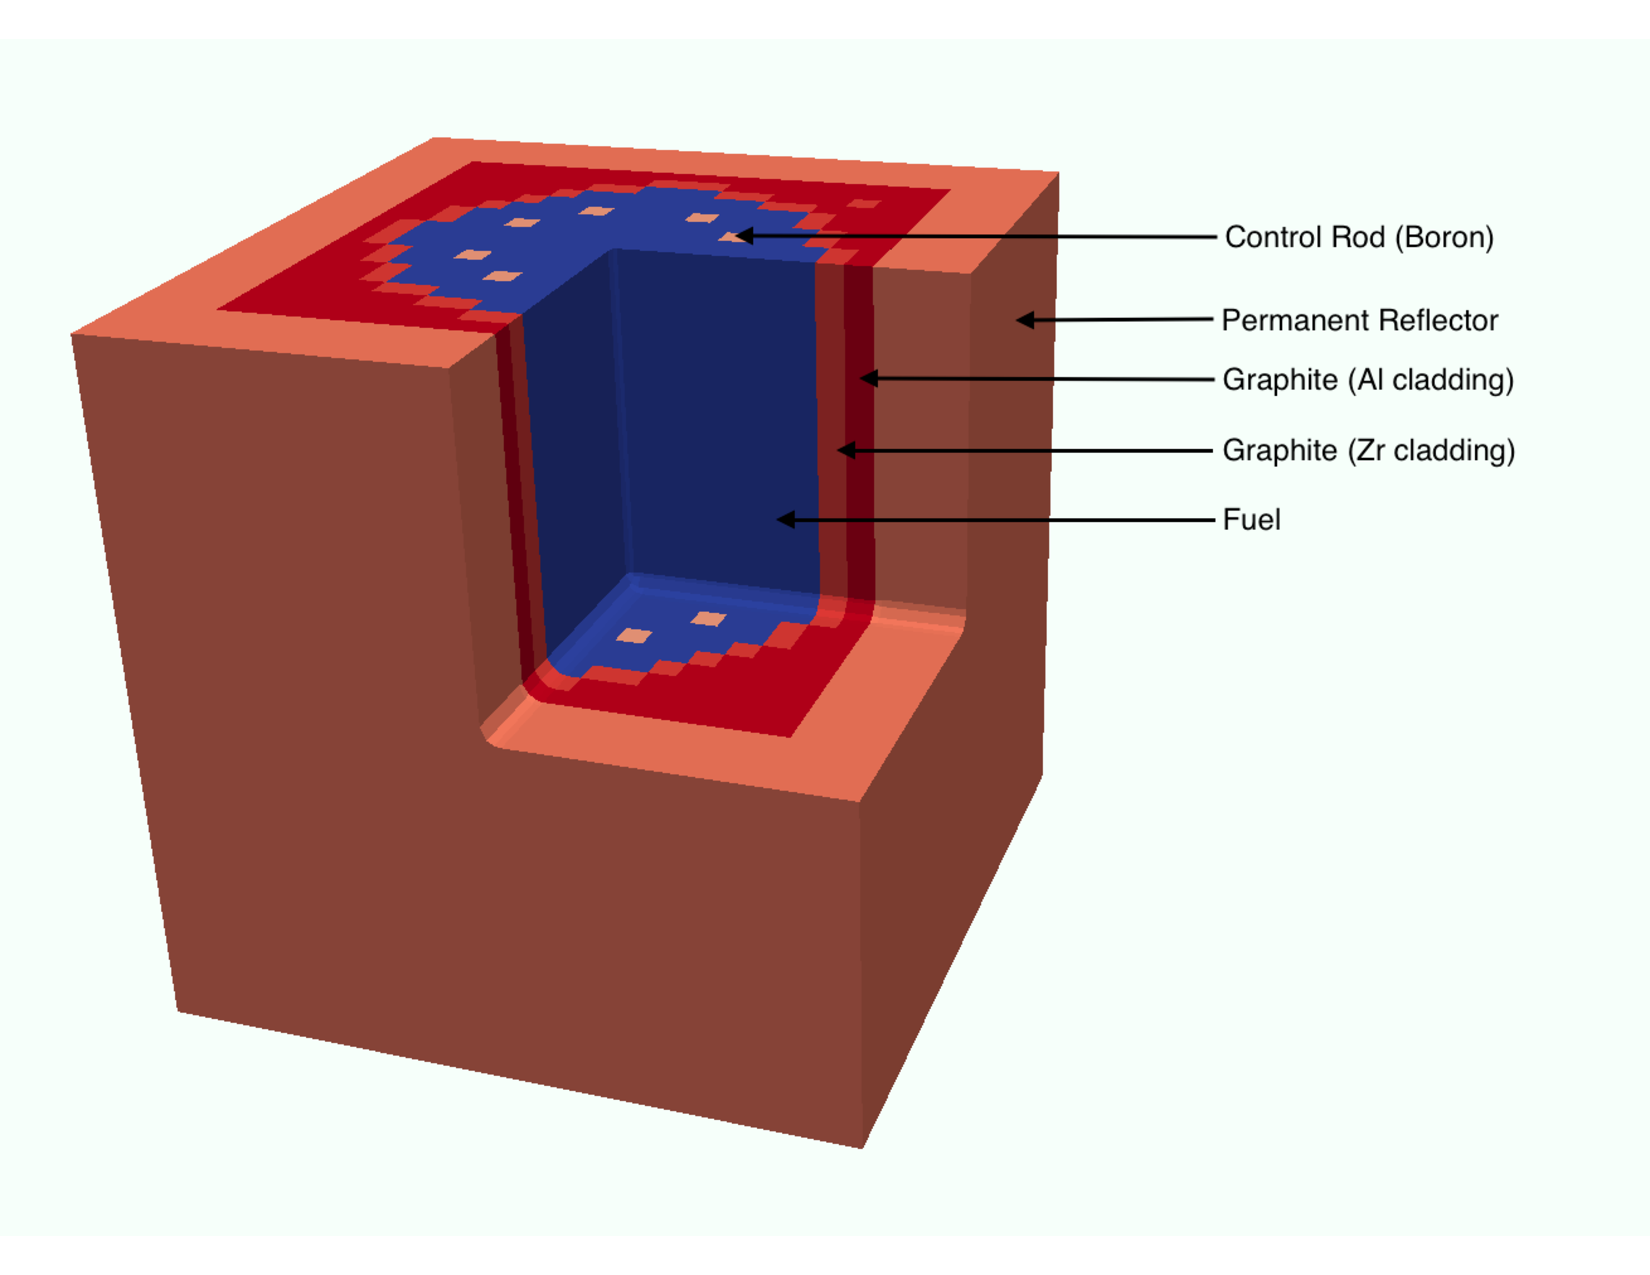
\includegraphics[scale=0.35]{./figures/transient-17.pdf}
  \caption{Geometry of the Transient-17 model. \label{fig:treat_macro}}
\end{figure*}

A trace of the integrated reactor power versus time is depicted in Fig. \ref{}.

%%%%%%%%%%%%%%%%%%%%%%%%%%%%%%%%%%%%%%%%%%%%%%%%%%%%%%%%%%%%%%%%%%%%%%%%%%%%%%%%
\subsection{(b) UO2 pellet - Graphite model}\label{sec:micro_model}
The micro-structure model comprises three isotopes: $^{12}C$ in the region outside of the fuel particle, $^{235}U$ and $^{16}O$ within the fuel particle. A spherical fuel particle with representative fission fragment cascades and the utilized uranium concentration are depicted in Fig. \ref{fig:radiation_damage_radius}.
For avoiding Gibbs' phenomenon when projecting the concentration values onto an FEM mesh, it is essential to ensure a smooth transition of the concentration from one region to another. For this purpose, we use the following expressions assuming a spherical fuel particle:
\begin{align}\label{eq:smooth_transition}
   c_j(\vec{r})& = \frac{1}{2} \left( C_{in,j}  \left( 1 + B \right) + C_{out,j}\left( 1 -B \right)  \right) \nonumber \\
   T &= \tanh a \left( \frac{r}{R}  - \frac{R}{r} \right),
\end{align}
where $r$ is the distance from the centroid of the fuel particle, $R$ is the radius of the fuel particle, and the free parameter $a$ determines the slope of the transition and we select $a=8$. The parameters $C_{in,j}$ and $C_{out,j}$ are the asymptotic concentrations inside and outside the sphere, respectively. The full paper will generalize the shape of the fuel particle to ellipsoids.

The average minimum distance of two fuel particles can be estimated assuming (1) that the fuel particles are spherical and (2) the fuel is uniformly distributed. Using the fuel volume fraction $f = 1 : 2571 \approx 0.0004$ we can find that the number of fuel particles in a box of dimension $L$ is roughly:
\begin{equation}
  N \approx \left( \frac{L^3 f}{4/3 \pi R^3} \right)^{1/3}.
\end{equation}
Following \cite{averagedistance}, a rough approximation of the average minimum distance between two particles in a box of dimension $L$ is:
\begin{equation}
   <r> \approx \left( \frac{L^3}{N} \right)^{1/3} = \left(\frac{4}{3} \frac{\pi}{f} \right)^{1/3} r \approx 22 R. 
\end{equation}
(Note: Pedram has the factor $0.896/(f)^{1/3}$). The average minimum distance between fuel particles is typically much larger than the range of fission fragments. Therefore, the size of the micro-structure domain can be chosen conveniently as long as the boundaries conditions are far enough away from the fuel so they do not influence the heat conduction or allow escape of fission fragments.
The micro-scale heat conduction problem and the rasterization is performed on a uniform, three-dimensional, hexahedral mesh comprising 1,000,000 elements. This is necessary to accurately represent the surface of the spherical fuel particle.

The typical relaxation time scale $\tau$ for a TREAT fuel particle is much smaller than the macroscopic time step. It can be estimated to be:
\begin{equation}
   \tau = \frac{R^2 c_p \rho}{k \pi^2} \approx  \cdot 10^{-5}-10^{-4} s.
\end{equation}
Hence the temperature distribution can be assumed to be in quasi-steady state at each neutronics timestep. 

\begin{figure}[t] % replace 't' with 'b' to force it to be on the bottom
  \centering
  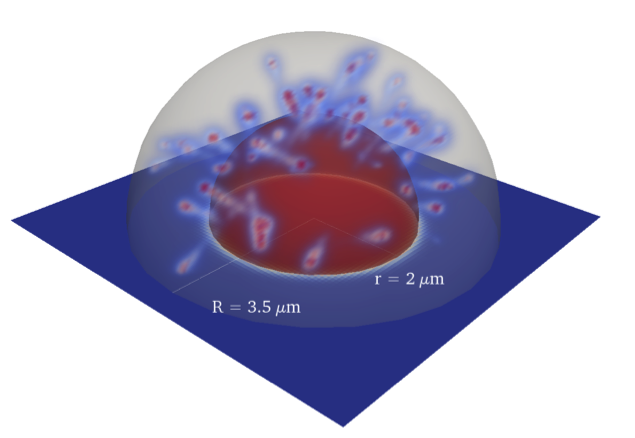
\includegraphics[scale=0.6]{./figures/radiation_damage_radius.png}
  \caption{Fission fragement sample trajectories overlayed on fuel particle with radius $r=20 \mu m$. The $^{235}U$ concentration is plotted in the projected plane. A transparent sphere of radius $r=35 \mu m$ is added to assess typical distances fission fragments travel into the graphite matrix. \label{fig:radiation_damage_radius}}
\end{figure}

\subsection{Numerical Results}


%%%%%%%%%%%%%%%%%%%%%%%%%%%%%%%%%%%%%%%%%%%%%%%%%%%%%%%%%%%%%%%%%%%%%%%%%%%%%%%%
\section{Conclusions and Future Work}
to-come

%%%%%%%%%%%%%%%%%%%%%%%%%%%%%%%%%%%%%%%%%%%%%%%%%%%%%%%%%%%%%%%%%%%%%%%%%%%%%%%%
\section{Acknowledgments}
This work is supported by the U.S. Department of Energy, under DOE Idaho Operations Office Con- tract DE-AC07-05ID14517. Accordingly, the U.S. Government retains a nonexclusive, royalty-free license to publish or reproduce the published form of this contribution, or allow others to do so, for U.S. Government purposes.

%%%%%%%%%%%%%%%%%%%%%%%%%%%%%%%%%%%%%%%%%%%%%%%%%%%%%%%%%%%%%%%%%%%%%%%%%%%%%%%%
\begin{thebibliography}{1}

\bibitem{treat} U.S. Department of Energy, {\em Mission Need Statement for the Resumption of Transient Fuel Testing}, U.S. DOE, December 3, 2010. \\

\bibitem{Mo2015} Kun Mo et al., {\em Heat transfer simulations of the UO2 particle-graphite system in TREAT fuel}, Nuclear Engineering \& Design, Vol. 293, November, 2015. \\

\bibitem{DeHart2016} Mark DeHart et al., {\em RESEARCH IN SUPPORT OF TREAT KINETICS CALCULATIONS USING RATTLESNAKE/BISON COUPLING WITHIN MAMMOTH}, Physor 2016 -Unifying Theory and Experiments in the 21st Century, Sun Valley, ID, USA, May, 2016. \\

\bibitem{TreatFeedback} Javier Ortensi et al.,  {\em Full Core TREAT Kinetics Demonstration Using Rattlesnake/BISON Coupling Within MAMMOTH}, Research report INL/EXT-15-36268, Idaho National Laboratory, Idaho Falls, Idaho, August 2015.\\

\bibitem{DH} James J. Duderstadt and Louis J. Hamilton, {\em Nuclear Reactor Analysis}, John Wiley \& Sons, 1976.\\

\bibitem{GammaHeating} Y.K. Lee, J.-C. David, and H. CarCreff, {\em A Gamma Heating Calculation Methodology for Research Reactor Applications}. in Proc. 5th ENS Int.Topical Meeting Research Reactor Fuel Management, Aachen, Germany, Apr. 1-3, 2001.\\

\bibitem{SRIM} J. F. Ziegler and J. P. Biersack and M. D. Ziegler (2008). SRIM - The Stopping and Range of Ions in Matter. SRIM Co. ISBN 0-9654207-1-X.\\

\bibitem{COMSOL} {\em COMSOL Multiphysics 4.3b,} User's guide, COMSOL Inc.\\

\bibitem{Moose} H. Park, D. Knoll, D. Gaston, and R. Martineau, {\em Tightly Coupled Multiphysics Algorithms for Pebble Bed Reactors,} Nuclear Science and Engineering, Vol. 166(2), pp. 118-133, 2010.\\

\bibitem{MyTRIM} Daniel Schwen et al., {\em Molecular dynamics simulation of intragranular Xe bubble re-solution in UO 2}, Journal of Nuclear Materials, Vol. 392, 2009.\\

\bibitem{MAMMOTH} Mark DeHart, {\em TREAT Modeling and Simulation Development with Validation Requirements} Research report INL/CON-15-36200, Idaho National Laboratory, Idaho Falls, Idaho.\\

%\bibitem{basics} Mark T. Robinson, {\em Basic physics of radiation damage production}
%Journal of Nuclear Materials 216 (1994) 1-28 \\
%
%\bibitem{BCA} R. Smith (ed.) {\em Atomic and ion collisions in solids and at surfaces:
% theory, simulation and applications}, Cambridge University Press, Cambridge, UK,
%  1997 \\

\bibitem{ENDFManual} The Members of the Cross Sections Evaluation Working Group, {\em ENDF-6 Formats Manual}, Research Report, Brookhaven National Laboratory,
BNL-90365-2009, Upton, NY, June, 2009.  \\

\bibitem{geant} GEANT4 Physics Manual Version: 10.2 (4 December 2015). \\

\bibitem{averagedistance} Bhattacharyya, P., and B. K. Chakrabarti. The mean distance to the nth neighbour in a uniform distribution of random points: an application of probability theory. Eur J. Phys. 29, pp. 639-645.\\

%\bibitem{Rattlesnake} Y. Wang et al., {\em Rattlesnake: User Manual}, Technical Report, Idaho National Laboratory, Idaho Falls, ID, 2016. 

\end{thebibliography}



\end{document}
